
% CVPR 2023 Paper Template
% based on the CVPR template provided by Ming-Ming Cheng (https://github.com/MCG-NKU/CVPR_Template)
% modified and extended by Stefan Roth (stefan.roth@NOSPAMtu-darmstadt.de)

\documentclass[10pt,twocolumn,letterpaper]{article}

%%%%%%%%% PAPER TYPE  - PLEASE UPDATE FOR FINAL VERSION
%\usepackage[review]{cvpr}      % To produce the REVIEW version
\usepackage{cvpr}              % To produce the CAMERA-READY version
%\usepackage[pagenumbers]{cvpr} % To force page numbers, e.g. for an arXiv version

% Include other packages here, before hyperref.

\usepackage{graphicx}
\usepackage{float}
\usepackage{amsmath}
\usepackage{amssymb}
\usepackage{booktabs}
\usepackage{subcaption} % Add subcaption package


% It is strongly recommended to use hyperref, especially for the review version.
% hyperref with option pagebackref eases the reviewers' job.
% Please disable hyperref *only* if you encounter grave issues, e.g. with the
% file validation for the camera-ready version.
%
% If you comment hyperref and then uncomment it, you should delete
% ReviewTempalte.aux before re-running LaTeX.
% (Or just hit 'q' on the first LaTeX run, let it finish, and you
%  should be clear).
\usepackage[pagebackref,breaklinks,colorlinks]{hyperref}


% Support for easy cross-referencing
\usepackage[capitalize]{cleveref}
\crefname{section}{Sec.}{Secs.}
\Crefname{section}{Section}{Sections}
\Crefname{table}{Table}{Tables}
\crefname{table}{Tab.}{Tabs.}


%%%%%%%%% PAPER ID  - PLEASE UPDATE
\def\cvprPaperID{*****} % *** Enter the CVPR Paper ID here
\def\confName{CVPR}
\def\confYear{2023}


\begin{document}

%%%%%%%%% TITLE - PLEASE UPDATE
\title{Tiny Image Generation}

\author{Viraj Chhajed\\
\and
Raayan Dhar
\and
Johnathan Harding
\and
William Zhou
}
\maketitle

%%%%%%%%% ABSTRACT
\begin{abstract}
This paper presents a study of small image size generative modeling using diffusion models and PixelCNN. Our experiments are focused on two `tiny image' datasets, optimized for our computational constraints. By analyzing the interpolation in our diffusion models, investigating various beta and noise schedules, and evaluating the denoising capabilities at different sampling steps, we provide novel insights into the mechanisms and effectiveness of each model type.

We measure the quality of generated images using FID scores and validate model performance through qualitative and quantitative assessments. The outcomes of this study illuminate the strengths and limitations of each approach, with particular attention to the adaptation of diffusion models for small image sizes. The results have promising implications for the application of these models in domains where computational efficiency is paramount.
\end{abstract}

%%%%%%%%% BODY TEXT
\section{Introduction}
\label{sec:intro}

Historically, the post-CNN image generation paradigm has developed into a branching field spanning many model types, including PixelCNNs, Generative Adversarial models, diffusion models, score-based models, and normalizing-flow based models. In this paper, we explore the performance of Pixel Convolutional Neural Networks (PixelCNNs) \cite{PixelCNN}, Denoising Diffusion Probabilistic Models (DDPMs) \cite{DDPM}, and Denoising Diffusion Implicit Models (DDIMs) \cite{DDIM} for image generation tasks. 

\hfill

PixelCNNs, as a form of autoregressive model, capitalize on the spatial hierarchical structure of images to predict pixel values sequentially. On the other hand, DDPMs and DDIMs, both rooted in the framework of diffusion models, represent a class of generative models that transform a distribution of random noise into a distribution of coherent images through a process of gradual denoising. DDPMs iteratively refine this process through a fixed number of steps, while DDIMs propose an accelerated approach, allowing for faster convergence with fewer steps without compromising the quality of the generated images. By comparing these models, we aim to shed light on their image-generation abilities by examining their output visual quality, speed, and flexibility. We quantitatively measure quality via the FID (Frechet Inception Distance) score metric \cite{FID}.

%-------------------------------------------------------------------------
\section{Results}
\subsection{PixelCNN}
Our PixelCNN results demonstrated the profound difficulty of image generation with smaller, older architectures. While we were unable to replicate the quality of our diffusion results with PixelCNN, our model achieved some representation of the spatial relationship between different colors and what appears to be edge detection/background vs. foreground, as shown in [\ref{fig:pixelcnnsamples}]. We achieved significantly reduced $L_1$ loss (from 58.4 to about 0.14) after a single epoch, and then had an difficult time reducing loss further. We were able to reach minimum $L_1$ losses of around 0.05 when we trained on a single image for 450000 iterations in an effort to assess the capacity of the PixelCNN to learn on an invariant input. 

\subsection{DDPM}
The DDPM models performed qualitatively well, generating realistic images when trained on both the CIFAR-10 [\ref{fig:beta_schedules}] and Anime-Faces [\ref{subfig:500steps}] datasets. On the CIFAR-10 dataset, the best DDPM model achieved an FID score of 123.53 (using the sigmoid scheduler) whereas the best DDPM model on the Anime-Faces dataset achieved an FID score of 92.93. While these are not state-of-the-art, our DDPM implementation significantly outperforms random noise (FID of $\sim550$) and PixelCNN results and maintains high image quality on inspection.

\subsubsection{Beta Schedules}
\label{subsubsec:beta}
We used cosine [\ref{subfig:cosine_beta}], linear [\ref{subfig:linear_beta}], sigmoid [\ref{subfig:sigmoid_beta}] and quadratic [\ref{subfig:quadratic_beta}] beta schedules. We found that by far, the cosine beta scheduled formed the worst. We can visually see this in [\ref{subfig:cosine_beta}], as the generated images are of much worse quality, with very high contrast and saturation. 

\hfill

Furthermore, the FID score for the cosine beta schedule actually increased across sampling steps after the initial drops, which is unlike any of the other beta schedules, which all decreased across sampling steps. This suggests that the model is capable of doing the majority of its denoising work in a few steps, which lends credence to the idea that the cosine scheduler improves fast sampling performance, discussed further in [\ref{subsubsec:varschedinsight}]. The validation loss for the cosine beta schedule was also the highest at nearly all epochs [\ref{subfig:validloss}], but note that the sigmoid beta schedule hovered around the same values as well. The linear beta schedule had by far the lowest validation loss, being at least 0.01 lower on average.

\hfill

It is important to note that the validation loss isn't perfectly correlated with accuracy - the linear scheduler, despite having the best validation loss, performs the second-worst in terms of FID score. This indicates that a more accurate per-step noise estimate doesn't necessarily yield a better final denoising result.

\subsubsection{Sampling}
\label{subsec:sampling_results}


The quality of image samples increases with the number of DDIM sampling steps taken. Note the difference between [\ref{subfig:500steps}] and [\ref{subfig:5steps}]; the 500-step process generates images with significantly higher quality reflections, structure, and high-resolution details. This result is mirrored quantitatively in the CIFAR-10 FID scores [\ref{subfig:cifar10_fid}], where FID distances decrease as sampling steps increase (for all schedulers other than cosine). 

\section{Discussion}

\subsection{PixelCNN}
Image generation remains a non-trivial task to implement if one has access to limited computing power and model complexity. We realized the limitations of the PixelCNN to generate high-quality images when trained on the entirety of CIFAR-10, and therefore considered reducing the scope of the problem, first by training solely on images of a single class, and then by training on a single image alone. We include surprising output images [\ref{fig:pixelcnnsamples}] sampled after hundreds of thousands of iterations through a single image, but they are still unsatisfactory compared to what is known to be possible with similar architectures like the PixelRNN \cite{pixelrnn} or PixelCNN++ \cite{Salimans2017PixeCNN}. The prior includes more advanced recurrent stages, with LTSMs \cite{HochSchm97}, and PixelCNN++ included more advances improving weight initialization, adding layer normalization \cite{ba2016layer}, and a more advanced form of convolutional layers referred to as “gated” convolution. We hypothesize that in order to create a more powerful PixelCNN we would require significant architectural changes. The immediate change, unrelated to PRNN or PCNN++ is that that our base-line model is likely too small to operate at the level of our diffusion architectures, with less than 1\%  of the number of parameters of our DDPM implementation. Despite these results, we believe there was a tangible amount of learning, with a drastic reduction in L1 loss from the initialization of the model to after the first epoch (58.4 to ~0.14). This further supports the difficulty of training image generation models. We believe that our PixelCNN learns features from a potential mean image in the training set, as well as spatial relationships between colors. The `stripiness' in our images [\ref{fig:pixelcnnsamples}] may indicate some level of the representation of edges, and placement of green and pink in these images may indicate a level of foreground vs. background distinction.

\subsection{DDPMs}
DDPMs \cite{DDPM}, work on the principle of iteratively removing Gaussian noise from a pure-noise seed image. The training process of a DDPM model consists of two stages:

1. The forward (unparameterized) noise addition process, which gradually adds Gaussian noise to an image until only noise remains. We can formulate it as:
$$x_t = \sqrt{1 - \beta_t} x_{t-1} + \sqrt{\beta_t} \epsilon$$
Where $x_0$ is the initial image sampled from our data distribution, $\beta_t$ is the \textbf{variance schedule} at time $t$, and $\epsilon$ is an I.I.D noise sampled per timestep from $\sim \mathcal{N}(0, I)$. Intuitively, the variance schedule can be understood as the scale of the noise added at each timestep. Typically, $\beta_t$ increases with $t$, as the later stages in the forward diffusion process are intended to destroy most of the information in the original image.

Given that the summation of Gaussian random variables have additive variance, we can reformulate the above into this one-step equation:
$$x_t = x_0 \sqrt{\bar{\alpha}_t} + \epsilon\ (1 - \bar{\alpha}_t)$$

Where $\alpha_t = 1 - \beta_t$ and $\bar{\alpha}_t = \prod_{i=0}^t \alpha_t$. See [\ref{fig:noise_schedules}] for an illustration of the forward process.

\hfill

2. To train the model, we learn the noise added between $x_0$ and $x_t$. A typical training process goes as follows:
a. Sample a $t$ uniformly between $0$ and $T$. $T$ is the number of total forward (noise-adding) steps, which is a fixed value.
b. Calculate $x_t$ via the formulation above, and save $\epsilon$.
b. We train the model to predict $\epsilon_\theta(x_t, t)$. Note that the model's prediction is conditioned on $t$ via a positional embedding of the timestep.


\subsubsection{Variance Schedule Insight}
\label{subsubsec:varschedinsight}
It was shown in \cite{IDDPM} that the cosine beta scheduler is designed to retain significantly higher amounts of original image signal late in the noising process. This causes the task of extrapolating image features from noise to be significantly more difficult earlier in the process, which the authors discovered causes the model to perform better when denoising steps are skipped. However, this did not align with our results in [\ref{subsubsec:beta}]. In our case, it's likely our relatively small model was unable to learn the more challenging task that the cosine beta schedule posed. This phenomenon can be seen in the noise addition figures [\ref{subfig:cosine_noise}], where the cosine noise scheduler has significantly less noise at the $t = 750$ step than all the other schedulers.

\subsubsection{Loss Function Insight}

Effectively, our network is a learned denoiser trying to predict the exact noise \textbf{added to the image}. Specifically, the noise $\epsilon$ before being scaled by $\beta_t$ and added to $\sqrt{\bar{\alpha}_t} x_0$. We minimize the Huber loss \cite{HUBER} between $\epsilon_\theta$ and $\epsilon$:

$$\mathcal{L} =
    \left\{\begin{matrix}
        \frac{1}{2}(\epsilon - \epsilon_\theta)^{2} & \text{if} \ \left | (\epsilon - \epsilon_\theta)  \right | < 1\\
        (\epsilon - \epsilon_\theta) - \frac{1}{2} & \text{otherwise}
    \end{matrix}\right.$$
    
In the early stages of training, DDPM models trained with Huber Loss \cite{HUBER} produced significantly clearer images than those trained with $L_2$ loss and more diverse images than those trained with $L_1$ loss. The Huber loss acts as $L_2$ loss for elements of $\epsilon_\theta$ below 1, and acts identically to $L_1$ for elements above 1. We believe that the Huber loss aids stability by placing a cap on the gradient norm, while achieving diversity by providing a gentler gradient signal when the error is small.
\subsubsection{Denoising Insight}
In \cite{IDDPM}, it was shown that linear noise schedules work better for higher-resolution images, but for images of lower-resolution (i.e., $64 \times 64$ and $32 \times 32$) to be suboptimal. Namely, the authors claim that the linear noise schedule is too noisy at the end of the forward noise process, and thus using a noise schedule such as the cosine noise scheduling can be thought of as `reducing overfitting.' This was visually supported and discussed in our results [\ref{subsec:sampling_results}]. Further discussion of the sampling process can be found in [\ref{subsec:sampling}].

\hfill



\subsection{DDIMs}
\label{subsec:disc_ddims}
DDIM models \cite{DDIM} are DDPM models with a reformulated sampling process. This property allows us to train a singular model using the training loop discussed in the DDPM formulation \cite{DDPM} and sample from it using the DDIM formulation. We find DDIM sampling has two distinct advantages over DDPM sampling:

1. DDIM sampling can be \textbf{deterministic}. The injected noise, $z$, in the DDPM formulation causes the same latent image $x_T$ to yield different $x_0$s at the end of the sampling process between different sampling trials. On the other hand, DDIM processes have no stochasticity. This also implies a \textit{consistency} property, where a smooth walk in latent space yields a smooth walk in image space. We discuss this further in [\ref{sec:interpolation}].

2. DDIM sampling can take an \textbf{arbitrary number of steps}. A large speedup can be achieved by taking fewer denoising steps than the - typically quite large - number of noising steps. This speedup comes at a minor tradeoff with image quality, as shown in the FID vs Sampling Steps chart [\ref{subfig:cifar10_fid}].

\subsubsection{Interpolation} \label{sec:interpolation}
As shown in [\ref{fig:interpol}], a smooth interpolation between two latent noise images yields gradually transitioning images when the interpolated latents are denoised to image space. Note that the formulation for DDIM sampling [\ref{sec: DDIM_Sampling}] has no stochastic element, which causes the denoising process to establish a mapping between latent noise and generated image. This process is not possible for DDPM models; passing the exact same noises used for DDIM interpolation into the DDPM sampling process yields a completely different set of generated images [\ref{subfig:ddpm_interpol}].

\subsection{Further Work \& Limitations}
\subsubsection{Limitations}
Due to computational constraints, we did not try larger image sizes (e.g., 256 $\times$ 256), but we expect generated images from these large image size datasets to have even better quality. Furthermore, the FID score resizes images to be $299 \times 299$ using bilinear interpolation, so images of larger size will have more accurate FID scores.

\subsubsection{Further Work}
To improve the quality of our generations,  we were interested in investigating:
\begin{enumerate}
    \item Latent Diffusion Models (LDMS) \cite{LDMs}, where images are encoded and decoded via a VAE. Diffusion happens in latent space, making LDMs far more parameter and compute-efficient.
    \item PixelRNNs \cite{pixelrnn} and PixelCNN++ \cite{Salimans2017PixeCNN} to gain more insight into our PixelCNN's performance.
    \item Fourier positional embeddings, learned positional embeddings, and relative positional embeddings. 
    \item Class conditions via positional embeddings. We hypothesize that the DDIM denoising formulation will allow us to smoothly interpolate between class conditions, yielding an interesting semantic-space walk.
\end{enumerate}
 


\newpage
%%%%%%%%% REFERENCES
{\small
\bibliographystyle{ieee_fullname}
\bibliography{egbib}
}
\newpage
\section{Figures}
\begin{figure}[H]
    \centering
    \begin{subfigure}[b]{0.2\textwidth}
        \centering
        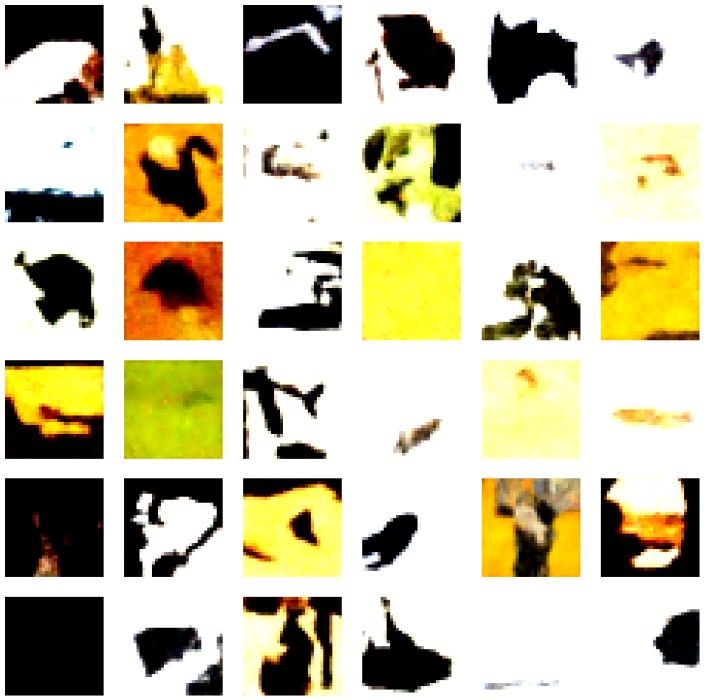
\includegraphics[width=\textwidth]{images_fixed/cifar10_cosine_beta.jpg}
        \caption{Cosine}
        \label{subfig:cosine_beta}
    \end{subfigure}
    \hfill
    \begin{subfigure}[b]{0.2\textwidth}
        \centering
        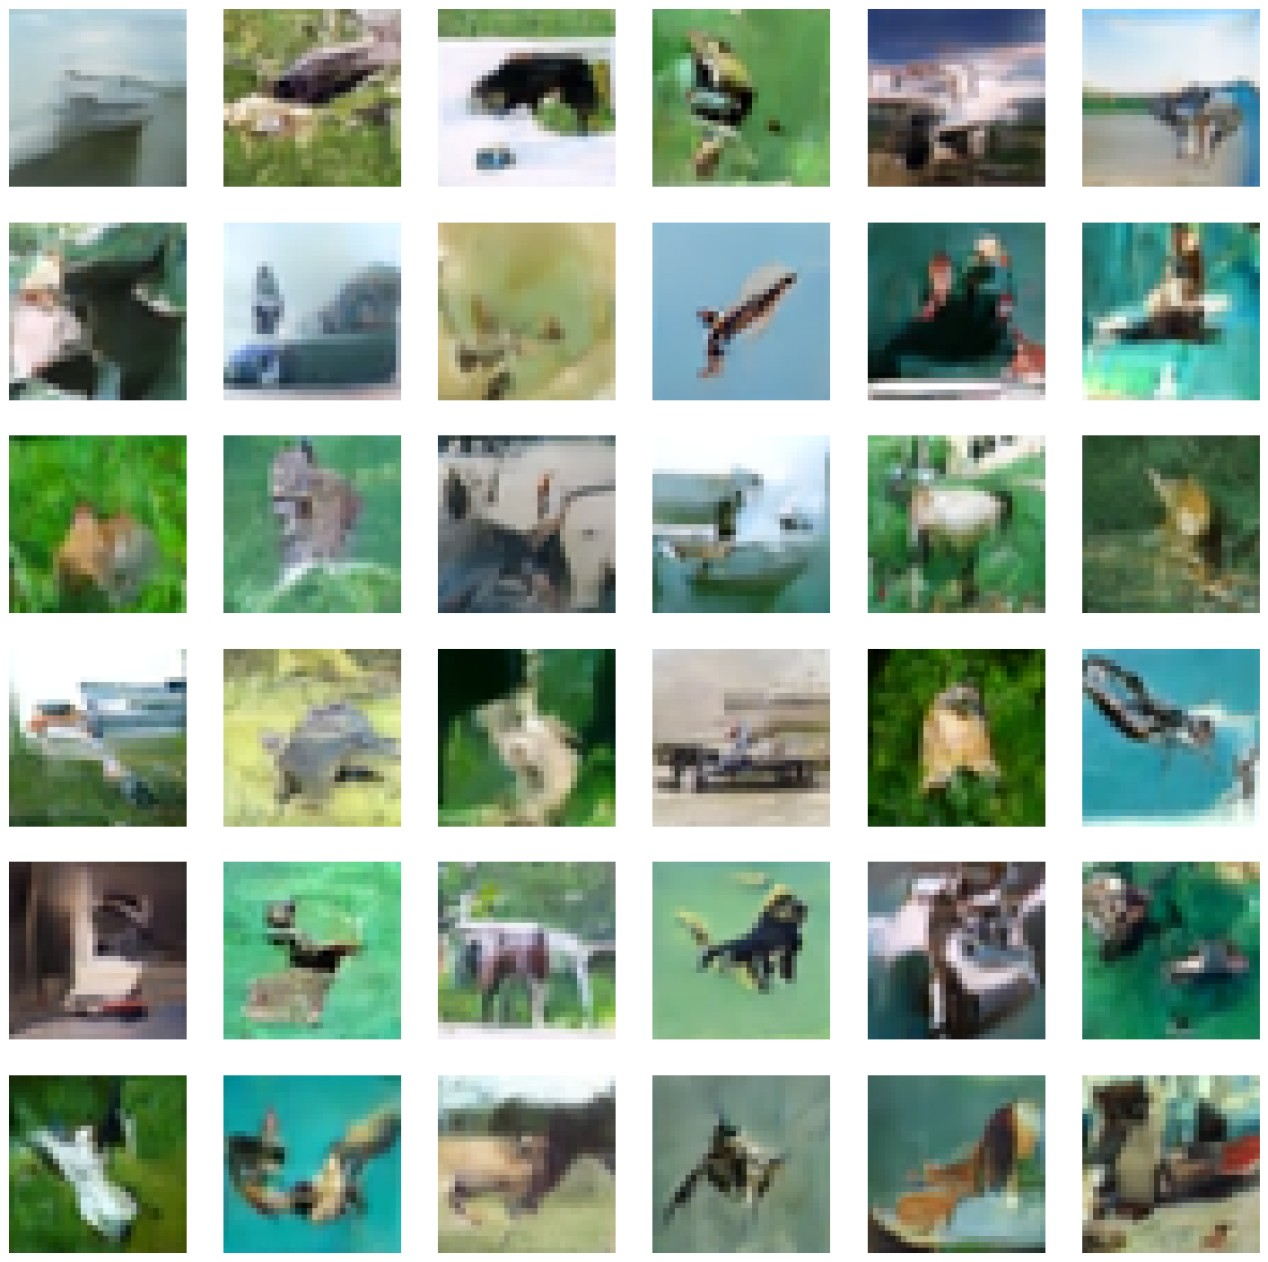
\includegraphics[width=\textwidth]{images_fixed/cifar10_linear_beta.jpg}
        \caption{Linear}
        \label{subfig:linear_beta}
    \end{subfigure}
    \hfill
    \begin{subfigure}[b]{0.2\textwidth}
        \centering
        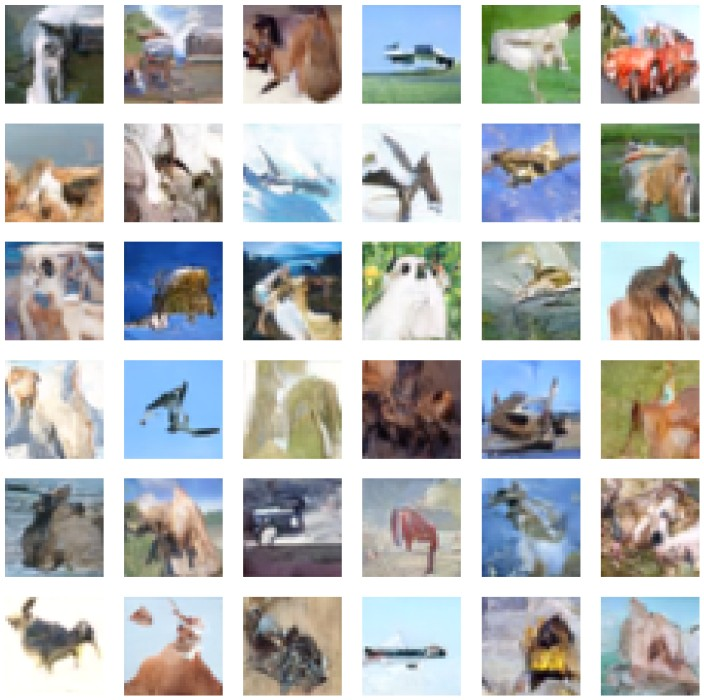
\includegraphics[width=\textwidth]{images_fixed/cifar10_sigmoid_beta.jpg}
        \caption{Sigmoid}
        \label{subfig:sigmoid_beta}
    \end{subfigure}
    \hfill
    \begin{subfigure}[b]{0.2\textwidth}
        \centering
        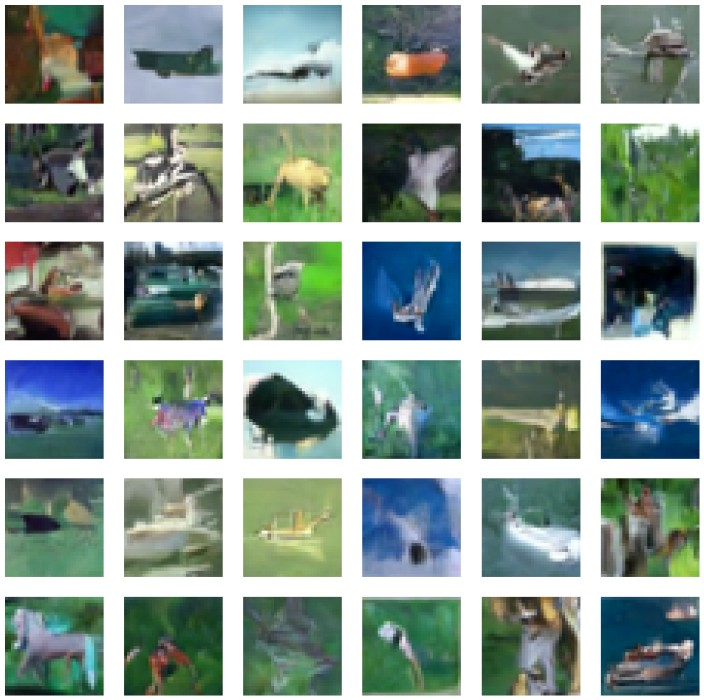
\includegraphics[width=\textwidth]{images_fixed/cifar10_quadratic_beta.jpg}
        \caption{Quadratic}
        \label{subfig:quadratic_beta}
    \end{subfigure}
    \caption{Beta schedules}
    \label{fig:beta_schedules}
\end{figure}
\begin{figure}[H]
    \centering
    \begin{subfigure}[b]{0.22\textwidth}
        \centering
        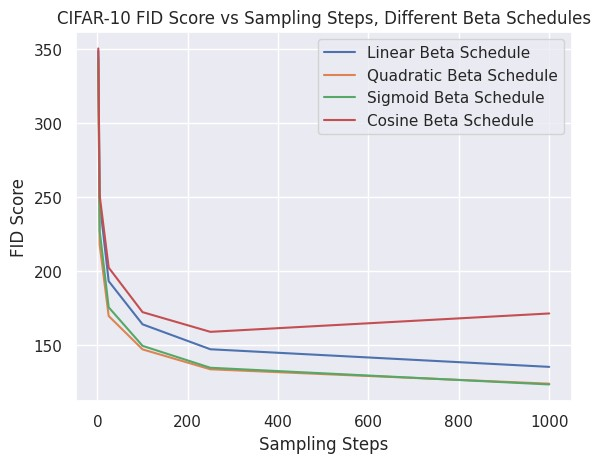
\includegraphics[width=\textwidth]{images_fixed/cifar10_FID.jpg}
        \caption{CIFAR10 FID Scores}
        \label{subfig:cifar10_fid}
    \end{subfigure}
    \hfill
    \begin{subfigure}[b]{0.22\textwidth}
        \centering
        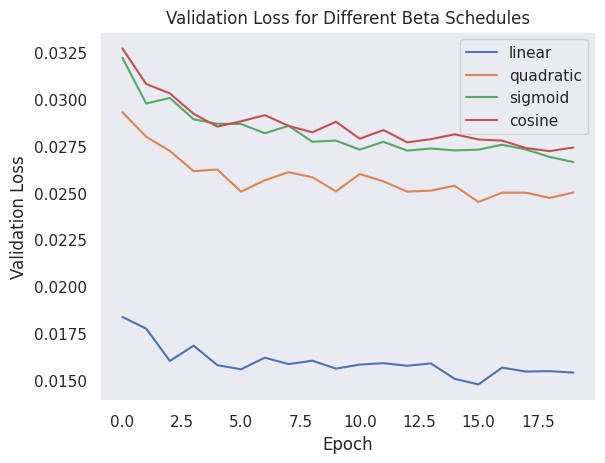
\includegraphics[width=\textwidth]{images_fixed/best_validloss.jpg}
        \caption{Validation Loss across Epochs among Different Beta Schedules}
        \label{subfig:validloss}
    \end{subfigure}
    \caption{Graphs}
    \label{fig:fidscores}
\end{figure}
\begin{figure}[H]
    \centering
    \begin{subfigure}[b]{0.22\textwidth}
        \centering
        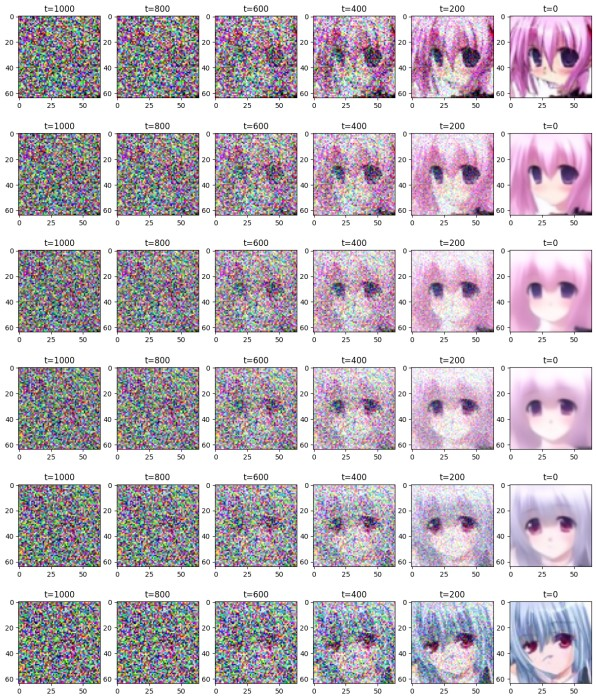
\includegraphics[width=\textwidth]{images_fixed/anime_interpol_ddim.jpg}
        \caption{DDIM Interpolation}
        \label{subfig:ddim_interpol}
    \end{subfigure}
    \hfill
    \begin{subfigure}[b]{0.22\textwidth}
        \centering
        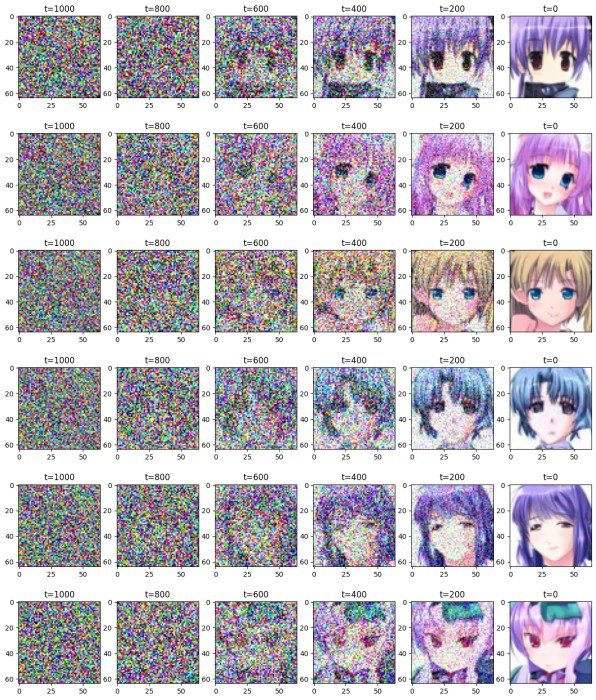
\includegraphics[width=\textwidth]{images_fixed/anime_interpol_ddpm.jpg}
        \caption{DDPM Interpolation}
        \label{subfig:ddpm_interpol}
    \end{subfigure}
    \caption{Interpolation}
    \label{fig:interpol}
\end{figure}
\begin{figure}
    \centering
    \begin{subfigure}[b]{0.4\textwidth}
        \centering
        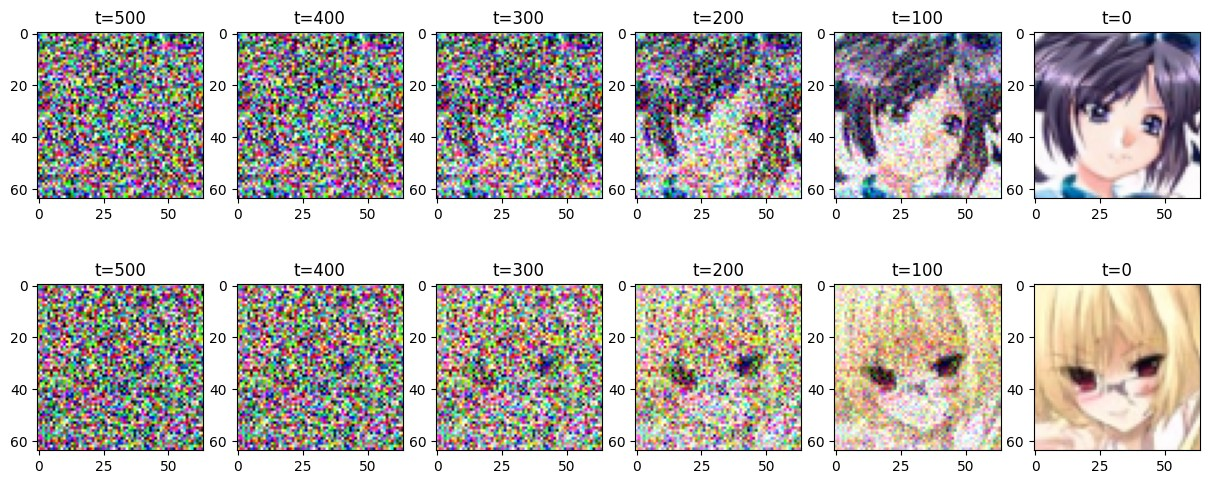
\includegraphics[width=\textwidth]{images_fixed/500_steps.jpg}
        \caption{500 Steps}
        \label{subfig:500steps}
    \end{subfigure}
    \hfill
    \begin{subfigure}[b]{0.4\textwidth}
        \centering
        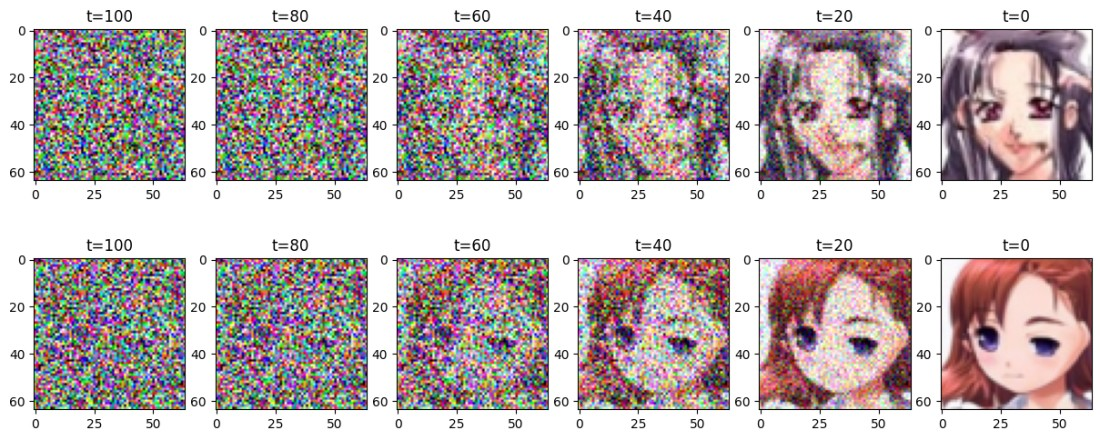
\includegraphics[width=\textwidth]{images_fixed/100_steps.jpg}
        \caption{100 Steps}
        \label{subfig:100steps}
    \end{subfigure}
    \hfill
    \begin{subfigure}[b]{0.4\textwidth}
        \centering
        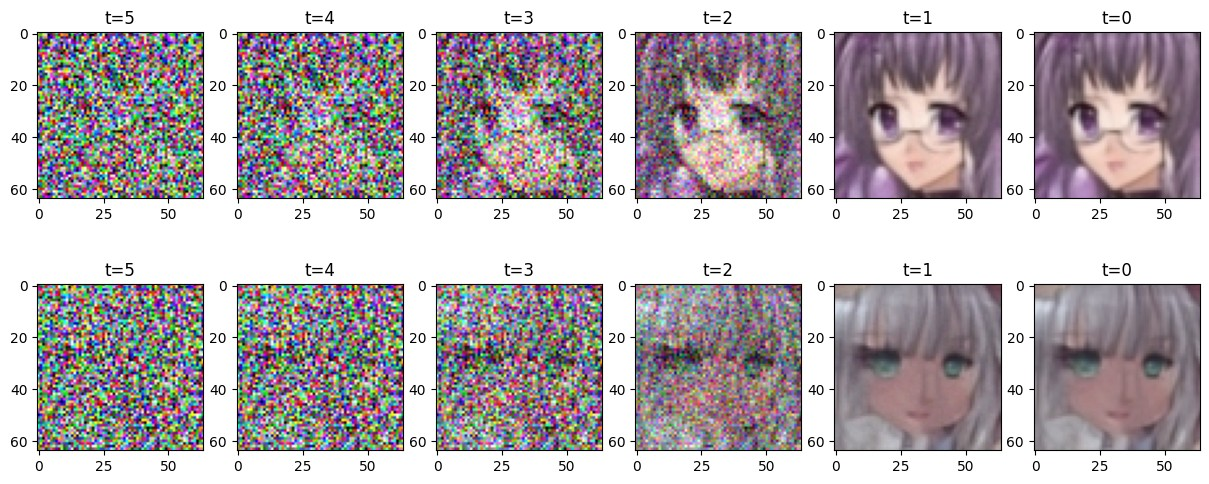
\includegraphics[width=\textwidth]{images_fixed/5_steps.jpg}
        \caption{5 Steps}
        \label{subfig:5steps}
    \end{subfigure}
    \caption{DDIM Denoising starting at different steps}
    \label{fig:steps}
\end{figure}
\begin{figure}
    \centering
    \begin{subfigure}[b]{0.4\textwidth}
        \centering
        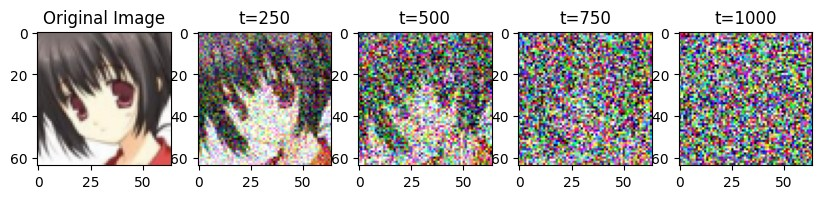
\includegraphics[width=\textwidth]{images_fixed/cosine_noise.jpg}
        \caption{Cosine}
        \label{subfig:cosine_noise}
    \end{subfigure}
    \hfill
    \begin{subfigure}[b]{0.4\textwidth}
        \centering
        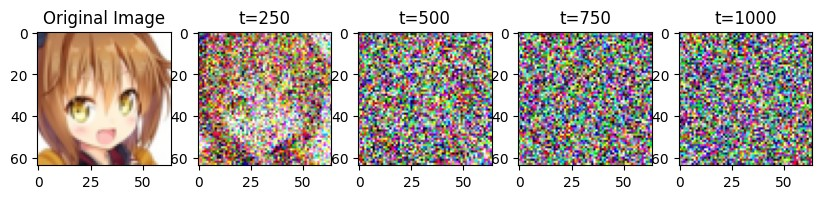
\includegraphics[width=\textwidth]{images_fixed/linear_noise.jpg}
        \caption{Linear}
        \label{subfig:linear_noise}
    \end{subfigure}
    \hfill
    \begin{subfigure}[b]{0.4\textwidth}
        \centering
        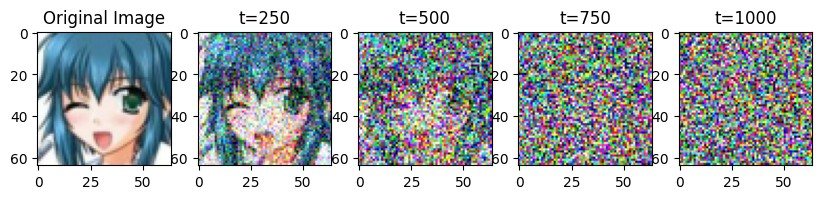
\includegraphics[width=\textwidth]{images_fixed/quadratic_noise.jpg}
        \caption{Quadratic}
        \label{subfig:quadratic_noise}
    \end{subfigure}
    \hfill
    \begin{subfigure}[b]{0.4\textwidth}
        \centering
        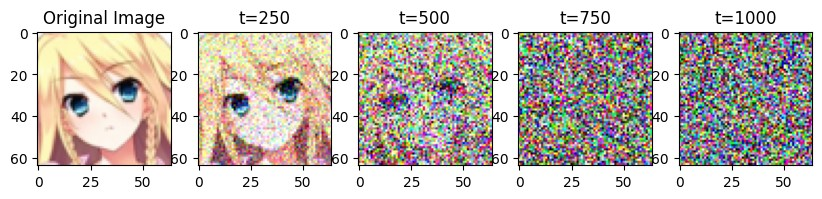
\includegraphics[width=\textwidth]{images_fixed/sigmoid_noise.jpg}
        \caption{Sigmoid}
        \label{subfig:sigmoid_noise}
    \end{subfigure}
    \caption{Forward Noise Scheduling}
    \label{fig:noise_schedules}
\end{figure}
\begin{figure}[H]
    \centering
    \begin{subfigure}[b]{0.09\textwidth}
        \centering
        
\includegraphics[width=\textwidth]{images_fixed/sample_50000.png}
        \label{subfig:sample50k}
        \caption{50k}
    \end{subfigure}
    \hfill
    \begin{subfigure}[b]{0.09\textwidth}
        \centering
        
\includegraphics[width=\textwidth]{images_fixed/sample_200000.png}
        \label{subfig:sample200k}
        \caption{200k}
    \end{subfigure}
    \begin{subfigure}[b]{0.09\textwidth}
        \centering
        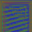
\includegraphics[width=\textwidth]{images_fixed/sample_250000.png}
        \label{subfig:sample250k}
        \caption{250k}
    \end{subfigure}
    \begin{subfigure}[b]{0.09\textwidth}
        \centering
        
\includegraphics[width=\textwidth]{images_fixed/sample_350000.png}
        \label{subfig:sample350k}
        \caption{350k}
    \end{subfigure}
    \begin{subfigure}[b]{0.09\textwidth}
        \centering
        
\includegraphics[width=\textwidth]{images_fixed/sample_450000.png}
        \label{subfig:sample450k}
        \caption{450k}
    \end{subfigure}
    \caption{PixelCNN Samples across Epochs Trained}
    \label{fig:pixelcnnsamples}
\end{figure}
\newpage
\section{Methods}
\subsection{Data}
We primarily trained on and report only two datasets, CIFAR10 \cite{Krizhevsky09} and an Anime Faces dataset from Kaggle \cite{Anime}. We chose these datasets since their image size was small and thus conducive to our limited computational resources. We downscaled the Anime Faces dataset to be 64 $\times$ 64. 
\subsection{U-Net}
\subsubsection{Training}
Outside of model choices (beta schedules, noise schedules, etc), we trained all our U-Nets on the entirety of the train partitions of their datasets for 20 epochs with batch size of 32, learning rate of $1\mathrm{e}{-4}$ and with 1000 forward steps. The total number of parameters was 171.39 million.
\subsubsection{Architecture}
Faithful to the DDPM paper \cite{DDPM}, we use a backbone of PixelCNN++ \cite{Salimans2017PixeCNN}, a U-Net \cite{DBLP:journals/corr/RonnebergerFB15} based on a Wide ResNet \cite{DBLP:journals/corr/ZagoruykoK16} with group normalization \cite{DBLP:journals/corr/GroupNorm} instead of batch normalization. However, we use weight-standardized ResNets which were empirically seen to work better with group normalization \cite{DBLP:journals/corr/WeightStandardization, DBLP:journals/corr/BiT}. Specifically, our model architecture consists of a time embedding, a down-sampling path, mid-level (bottleneck) blocks, and up-sampling paths. For our time embedding, we use a sinusoidal positional embedding layer to encode time step information \cite{NIPS2017_3f5ee243, DBLP:journals/corr/HendrycksG16}. This time embedding is passed through an MLP (linear $\rightarrow$ GeLU $\rightarrow$ linear) to obtain a time-dependent feature vector, which is then added to each residual block to enable the network to have knowledge of which particular time step it is operating. In our down-sampling path, we use two wide weighted-standardized ResNet blocks, followed by a linear attention \cite{katharopoulos-et-al-2020, shen2019efficient} layer which applies attention along the spatial dimensions and a convolution layer that reduces spatial dimensions by a factor of 2. After the down-sampling path, we use a wide weight-standardized ResNet block, followed by an attention block \cite{NIPS2017_3f5ee243} which applies attention along both the spatial and channel dimensions, followed by another wide weight-standardized ResNet block. Then, our up-sampling path consists of two wide weight-standardized ResNet blocks, followed by a linear attention block along the spatial dimensions and an up-sampling layer, which increases the spatial dimensions by a factor of 2 using nearest neighbor sampling. Finally, our feature maps from the up-sampling path are concatenated with the initial feature map, and a final wide weight-standardized ResNet block is applied to the concatenated feature maps. Then, a final convolutional layer is used to produce our output tensor.

\subsection{PixelCNN}
\subsubsection{Training}
We trained our PixelCNN on the entire CIFAR-10 dataset for up to 200 epochs as well as a single image for up to 450,000 epochs both with batch size of 32. Optimization primarily consisted of augmenting the number of training epochs, as we use the learning rate ($1\mathrm{e}{-3}$) employed by in the original PixelCNN paper \cite{PixelCNN, pixelrnn}. The total number of tunable parameters used was 1,307,651. 

\subsubsection{Architecture}
Inspired by \cite{PixelCNN, pixelrnn}, our PixelCNN is fundamentally based on a series of masked convolutions of an input image with size $3 \times 32 \times 32$. Our architecture included a total of four convolutional layers, two of which were masked to enforce an autoregressive structure. The output of each convolutional layer was followed by each of three stages, the feature maps produced by each convolutional batch-normalization layer \cite{DBLP:journals/corr/IoffeS15} followed by the ReLU activation layer. Our architecture also employed a residual stream \cite{elhage2021mathematical} (information travelling in the residual connections \cite{DBLP:journals/corr/HeZRS15}) incorporated at the end of the second masking  to prevent excessive information loss due to masking \cite{turukin_pixelcnn} though it is important to note that this architecture is not considered an RNN implementation. 

\subsection{Sampling}
\label{subsec:sampling}
\subsubsection{DDPM}\label{sec: DDPM_Sampling}
We reproduce the sampling process in the DDPM paper published by \textit{Ho et al}\cite{DDPM}. The reverse process, also known as the denoising process, begins with pure noise and iterates backward over $T$ steps.

$$x_T \sim \mathcal{N}(0, I)$$
$$x_{t-1} = \frac{1}{\sqrt{\alpha_t}} \left(x_t - \frac{1 - \alpha_t}{\sqrt{1 - \bar{\alpha}_t}} \epsilon_\theta(x_t, t)\right) + z \sqrt{\beta_t \frac{1 - \bar{\alpha}_{t-1}}{1 - \bar{\alpha}_t}}$$
Where $z \sim \mathcal{N}(0, I)$. 

\subsubsection{DDIM} \label{sec: DDIM_Sampling}
Mathematically, the DDIM sampling process is formulated as\cite{DDIM}:
$$x_{\tau_{i-1}} = \sqrt{\frac{\bar{\alpha}_{\tau_{i-1}}}{\bar{\alpha}_{\tau_i}}} \left(x_{\tau_i} - \sqrt{1 - \bar{\alpha}_\tau} \epsilon_\theta(x_{\tau_i}, \tau_i)\right)$$
$$+ \epsilon_\theta(x_{\tau_i}, \tau_i) \sqrt{1 - \bar{\alpha}_{\tau_{i-1}}}$$
Where $\tau$ is a series of monotonically increasing values spanning $0$ to $T$, inclusive. Note that $\tau$ does not have to correspond to $t$; $\tau = [0, 5, 10, ..., 1000]$ is also a valid sampling schedule.




\end{document}
